\chapter{Experimental Results and Discussion}
\label{ch:results}
\sloppy
\hbadness=8000

\section{Introduction}
This chapter presents and interprets the experimental results obtained by applying the methodology described in Chapter~III. The chapter is organised in the following sequence: experimental setup, dataset characteristics, model performance in both metric and imperial units, variance analysis by order size category, feature importance analysis, prediction validation on sample orders, 5-fold cross-validation stability, prediction error distribution, LSTM training convergence, season-wise and fabric-wise segmented performance, confidence interval coverage, and a synthesis discussion of key findings. Unless otherwise stated, all quantitative performance figures are reported on the held-out test set of 1{,}000 orders, which was not used in any stage of model training or hyperparameter selection.

\secdiv
\section{Experimental Setup}
All experiments were conducted on a workstation equipped with an Intel Core i7 processor (3.6\,GHz), 16\,GB RAM, and no dedicated GPU; all TensorFlow operations were executed on the CPU. The software environment comprised Python 3.10, scikit-learn 1.x for classical models and preprocessing, XGBoost 1.x for gradient boosting, and TensorFlow 2.x for the LSTM. All random number generators were seeded at 42 to ensure full reproducibility across runs. The complete training and evaluation pipeline---from data loading through metric computation and figure generation---completes in approximately 3.5 minutes on the described hardware, confirming that the system is practically deployable in factory IT environments without specialist compute infrastructure.

\secdiv
\section{Dataset Characteristics}

Table~\ref{tab:sample} presents five representative production orders drawn from the dataset to illustrate the structure of the input data. The orders span all five garment types and cover a range of order quantities from 500 to 2{,}500 units, fabric widths from 55 to 71 inches, and complexity levels from Simple to Complex. Comparing the Plan\,(yd) and Act\,(yd) columns reveals that the BOM formula over-plans for some orders (ORD\_03, Dress in Silk: plan 3{,}683\,yd vs.\ actual 3{,}598\,yd, a 2.4\% over-estimation) and under-plans for others (ORD\_04, Shirt in Polyester: plan 6{,}422\,yd vs.\ actual 6{,}589\,yd, a 2.5\% under-estimation), confirming the directional inconsistency of static BOM estimation even within a small sample.

\begin{table}[htbp]
\centering\scriptsize\tabcolsep=2pt\caption{Sample Production Dataset (5 representative orders)}\label{tab:sample}
{\hbadness=10000
\begin{tabularx}{\textwidth}{@{}C{1.6cm} Z >{\hsize=1.1\hsize}Y >{\hsize=0.8\hsize}Y >{\hsize=0.8\hsize}Y Z Y Y@{}}
  \toprule
  \textbf{ID}&\textbf{Garment}&\textbf{Fabric}&\textbf{Qty}&\textbf{W''}&\textbf{Cmplx}&\textbf{Plan(yd)}&\textbf{Act(yd)}\\
  \midrule
  ORD\_01&T-Shirt&Cotton&1.0k&63&Simple&1{,}452&1{,}488\\
  ORD\_02&Jacket&Denim&0.5k&71&Complex&3{,}119&3{,}241\\
  ORD\_03&Dress&Silk&0.8k&55&Medium&3{,}683&3{,}598\\
  ORD\_04&Shirt&Poly&2.5k&59&Medium&6{,}422&6{,}589\\
  ORD\_05&Pants&Blend&1.2k&63&Simple&4{,}242&4{,}189\\
  \bottomrule
\end{tabularx}
}
\end{table}

Across the full 5{,}000-order dataset, mean actual fabric consumption is 8{,}288\,yd (SD 5{,}688\,yd), reflecting the broad range of order scales from small bespoke runs of 100 units to high-volume commodity orders of 5{,}000 units. The mean planned BOM is 8{,}449\,yd, representing a systematic over-plan of 1.9\%. Approximately 42\% of orders over-consume relative to their BOM plan, while the remaining 58\% under-consume or exactly match---confirming that the BOM formula's 5\% safety buffer is not universally correct and can generate material procurement errors in both directions. The Pearson correlation between Order\_Qty and actual consumption is $r$=0.78, confirming that order quantity is the dominant numeric driver of fabric use. In contrast, marker efficiency shows only a weak negative correlation of $r$=$-$0.08 with actual consumption, indicating that efficiency variability in the 70--95\% operational range introduces noise that partially obscures the physics relationship.

\secdiv
\section{Model Performance Analysis}

Tables~\ref{tab:perf_m} and \ref{tab:perf_yd} report test-set performance for all five models in metres and yards respectively, alongside the BOM physics baseline. The results reveal a clear and consistent performance hierarchy that reflects each model's capacity to capture the non-linear consumption patterns present in the dataset.

\begin{table}[htbp]
\centering\footnotesize\caption{Performance --- Metres (1,000-order test set)}\label{tab:perf_m}
\begin{tabularx}{\textwidth}{@{}Z Y Y Y Y Y@{}}
  \toprule
  \textbf{Model}&\textbf{RMSE (m)}&\textbf{MAE (m)}&\textbf{R\textsuperscript{2}}&\textbf{MAPE}&\textbf{Time (s)}\\
  \midrule
  Linear Reg.&1{,}886&1{,}434&0.8669&49.28\%&0.8\\
  Random Forest&751&539&0.9789&15.92\%&12.4\\
  XGBoost&525&370&0.9897&8.14\%&3.6\\
  \textbf{LSTM Net}&\textbf{346}&\textbf{243}&\textbf{0.9955}&\textbf{5.14\%}&\textbf{33.0}\\
  Ensemble&385&263&0.9944&5.92\%&---\\
  \midrule\textit{BOM Base}&\textit{443}&\textit{296}&\textit{0.9927}&\textit{3.86\%}&\textit{---}\\
  \bottomrule
\end{tabularx}
\end{table}

\begin{table}[htbp]
\centering\footnotesize\caption{Performance --- Yards (1,000-order test set)}\label{tab:perf_yd}
\begin{tabularx}{\textwidth}{@{}Z Y Y Y Y Y@{}}
  \toprule
  \textbf{Model}&\textbf{RMSE (yd)}&\textbf{MAE (yd)}&\textbf{R\textsuperscript{2}}&\textbf{MAPE}&\textbf{vs.\ BOM RMSE}\\
  \midrule
  Linear Reg.&2{,}062&1{,}568&0.8669&49.28\%&---\\
  Random Forest&821&589&0.9789&15.92\%&---\\
  XGBoost&574&404&0.9897&8.14\%&---\\
  \textbf{LSTM Net}&\textbf{379}&\textbf{265}&\textbf{0.9955}&\textbf{5.14\%}&\textbf{$\approx$22\%}\\
  Ensemble&422&288&0.9944&5.92\%&Robust\\
  \midrule\textit{BOM Base}&\textit{484}&\textit{324}&\textit{0.9927}&\textit{3.86\%}&Baseline\\
  \bottomrule
\end{tabularx}
\end{table}

Linear Regression performs poorest across all metrics (RMSE 2{,}062\,yd, MAPE 49.28\%, R\textsuperscript{2}=0.8669), confirming that the relationship between order attributes and fabric consumption is strongly non-linear. The model's single-coefficient representation cannot capture the multiplicative interaction between garment type and order quantity, leading to catastrophic errors on high-volume complex garments where the linear extrapolation diverges sharply from actual consumption. Random Forest achieves a substantial improvement (RMSE 821\,yd, R\textsuperscript{2}=0.9789), demonstrating that ensemble tree methods handle non-linearity effectively; however, residual errors at large order scales remain significant due to the averaging of diverse tree predictions. XGBoost reduces RMSE further to 574\,yd (R\textsuperscript{2}=0.9897), with the regularised sequential boosting approach focusing progressive tree fitting on the hardest-to-predict residuals, yielding the best performance among tree-based methods at a modest training time of 3.6\,s.

LSTM achieves the lowest RMSE of 379\,yd (346\,m), MAE of 265\,yd, and the highest R\textsuperscript{2}=0.9955, establishing it as the best single model. The LSTM's advantage over XGBoost reflects its ability to model high-order feature interactions through recurrent hidden states---capturing the multiplicative garment$\times$quantity$\times$complexity relationship more precisely than gradient-boosted piecewise-constant trees. Its training time of 33.0\,s is approximately 9$\times$ longer than XGBoost but remains practical for weekly or seasonal retraining schedules. The Ensemble (R\textsuperscript{2}=0.9944, RMSE 422\,yd, MAPE 5.92\%) underperforms the LSTM slightly in point accuracy, as the inclusion of weaker base models (LR, RF) introduces some noise into the weighted average. However, the ensemble provides an important practical advantage: by combining models with diverse error modes, it mitigates the risk of the rare but costly catastrophic prediction failures that any single model can produce on atypical order configurations.

Against the BOM baseline (RMSE 484\,yd), the LSTM achieves a 21.8\% RMSE reduction and a superior MAE of 265\,yd versus the BOM's 324\,yd. It is notable that the BOM achieves a lower MAPE (3.86\%) than the LSTM (5.14\%). This apparent reversal occurs because the BOM's 5\% safety buffer is well-calibrated for \textit{average}-scale orders, suppressing percentage errors on typical orders while simultaneously causing larger absolute errors on outlier orders. The RMSE metric, which penalises large errors quadratically, is therefore the more operationally relevant performance measure, as it best captures the cost impact of high-value procurement mistakes.

\begin{figure}[htbp]
\centering

\includegraphics[width=\linewidth]{Chap4/fig_rmse}
\caption{Forecasting Model RMSE Comparison (yards, 1{,}000-order test set)}
\label{fig:rmse}
\end{figure}

Figure~\ref{fig:rmse} visualises the complete RMSE hierarchy. The progressive reduction from LR (2{,}062\,yd) through RF (821\,yd), XGBoost (574\,yd), and the BOM (484\,yd) to the LSTM (379\,yd) illustrates both the five-fold performance gain from moving to deep learning and the meaningful headroom the LSTM achieves over the physics baseline. The ensemble, positioned at 422\,yd, sits between the BOM and LSTM, offering a conservative but robust option for procurement-critical applications.

\secdiv
\section{Variance Analysis}
\label{sec:variance}

Understanding the directional bias in fabric consumption errors is as operationally important as measuring their magnitude. A model that makes only symmetric random errors is fundamentally different---and more manageable---from one that consistently over- or under-predicts for specific order types. Table~\ref{tab:variance} stratifies the full 5{,}000-order dataset by order quantity range and reports the mean planned BOM, mean actual consumption, mean absolute variance in yards, and mean variance as a percentage of plan.

{\footnotesize
\begin{table}[htbp]
\centering\caption{Consumption Variance Analysis}\label{tab:variance}
\begin{tabularx}{\textwidth}{@{}L{2.8cm} C{1.5cm} C{2.2cm} C{2.2cm} C{2.2cm} X@{}}
  \toprule
  \textbf{Qty Range}&\textbf{Count}&\textbf{Plan(yd)}&\textbf{Act(yd)}&\textbf{Var(yd)}&\textbf{Var(\%)}\\
  \midrule
  100--500&392&963.6&1{,}005.4&+41.8&+4.49\%\\
  501--1.5k&1{,}000&3{,}299&3{,}362&+62.5&+2.04\%\\
  1.5k--3k&1{,}533&7{,}474&7{,}404&$-$70.6&$-$0.83\%\\
  3k--5k&2{,}075&13{,}065&12{,}691&$-$374.1&$-$2.79\%\\
  \midrule\textbf{All}&\textbf{5,000}&---&---&---&$\approx$0\%\\
  \bottomrule
\end{tabularx}
\end{table}
}

The results reveal a systematic and monotonic size-dependent bias: small orders (100--500 units) consistently \textit{over-consume} fabric relative to their BOM plan by an average of $+$4.49\%, while large orders (3{,}000--5{,}000 units) systematically \textit{under-consume} by $-$2.79\%. This pattern arises from the physics formula's handling of fixed-cost waste components. For small orders, the per-unit contribution of fabric allocated for cutting-line setup, selvedge waste, and end-of-roll remnants is proportionally large relative to the productive fabric in the marker, causing actual consumption to exceed the formula's per-unit estimate. Conversely, for large orders these fixed waste components are amortised across a greater number of units, and the improvements in marker efficiency achievable at scale push actual consumption below the BOM prediction. The 501--1.5k unit range shows a mild over-consumption of $+$2.04\%, while the 1.5k--3k range approaches near-neutrality ($-$0.83\%), indicating that the BOM formula is most accurately calibrated for mid-range production runs.

Across all 5{,}000 orders the mean variance is approximately zero (mean $-$0.65\%), confirming that the dataset is globally unbiased in aggregate. However, from a procurement planning perspective, the size-dependent directionality is operationally significant. A factory whose seasonal programme is dominated by small bespoke orders should expect to consume approximately 4.5\% more fabric than the BOM suggests, and should therefore procure accordingly. A factory with a high proportion of large commodity orders, conversely, should expect to procure approximately 2.8\% less than the BOM recommends. The ML models, trained on historical data that encodes these order-size-dependent patterns, are substantially better positioned than the static BOM formula to issue directionally correct fabric requirements across the full order-size spectrum.

\begin{figure}[htbp]
\centering

\includegraphics[width=0.80\linewidth]{Chap4/fig_variance}
\caption{Planned vs.\ Actual Consumption Variance (\%) by Order Quantity Range}
\label{fig:variance}
\end{figure}

Figure~\ref{fig:variance} plots the mean variance percentage for each order-quantity band, illustrating the monotonic transition from over-consumption at small scale to under-consumption at large scale. The crossing point at approximately 1{,}500 units identifies the order size at which the BOM formula is most accurate. This threshold provides a practical guideline for planners deciding when to apply a manual correction to BOM estimates in the absence of ML tooling.

\secdiv
\section{Feature Importance Analysis}
\label{sec:fi}

XGBoost's gain-based feature importance scores, reported in Table~\ref{tab:fi} and visualised in Figure~\ref{fig:fi}, reveal that fabric consumption prediction is driven by a small number of dominant features, with the remaining features contributing incrementally. The gain metric measures the average improvement in accuracy brought by each feature when it is used in a tree split, normalised so that all scores sum to 1.0.

\begin{table}[htbp]
\centering\footnotesize\tabcolsep=4pt\caption{Feature Importance --- XGBoost Model}\label{tab:fi}
\begin{tabularx}{\textwidth}{@{}C{0.8cm} Z Y Y Z@{}}
  \toprule
  \textbf{Rnk}&\textbf{Feature}&\textbf{Imp.}&\textbf{Cum.}&\textbf{Implication}\\
  \midrule
  1&Garment Type&0.518&52\%&Base consumption varies 3$\times$\\
  2&Order Quantity&0.297&81.5\%&Non-linear scale effect\\
  3&Pattern Complexity&0.102&92\%&Complexity mult.\ 1.0--1.35\\
  4&Fabric Width&0.039&96\%&Wider = fewer yd/unit\\
  5&Marker Eff\%&0.011&97\%&Higher = less waste\\
  6&Operator Exp&0.010&98\%&Reduces over-consumption\\
  7&Defect Rate\%&0.009&99\%&Re-cutting multiplies consumption\\
  8&Season&0.007&99\%&Small seasonal offset\\
  9&Fabric Type&0.007&100\%&Minimal direct impact\\
  \bottomrule
\end{tabularx}
\end{table}

Garment type is the single most important predictor (importance score 0.518, 52\% of total gain), reflecting the fundamental physical reality that jacket fabric consumption ($\approx$3.5--5\,yd/unit for a complex winter jacket) is roughly three to four times that of a T-shirt ($\approx$0.9--1.2\,yd/unit), and that these garment-class differences are the largest source of consumption variance in the dataset. Order quantity ranks second (0.297, cumulative 82\%), capturing the non-linear scale relationship in which doubling order size does not double fabric consumption proportionally---because higher-volume orders benefit from better marker utilisation rates. Together, garment type and order quantity account for 81.5\% of the model's total split gain, confirming that any fabric consumption forecasting system must first and foremost be garment-type-aware and quantity-sensitive.

Pattern complexity contributes a meaningful 10.2\% (rank~3), consistent with its role as a direct consumption multiplier in the physics formula (Simple=1.0, Medium=1.15, Complex=1.35). Fabric width (rank~4, 3.9\%) captures the inverse relationship between bolt width and required fabric length per unit: wider fabric reduces yardage requirements for any given marker. The remaining five features---marker efficiency, operator experience, defect rate, season, and fabric type---each contribute less than 1.2\% individually. While these contributions are small relative to garment type and quantity, they are not negligible for high-precision procurement at scale; collectively they represent the stochastic production-quality dimension of fabric consumption.

\begin{figure}[htbp]
\centering

\includegraphics[width=0.92\linewidth]{Chap4/fig_fi}
\caption{Feature Importance --- XGBoost Model (higher score = more influential predictor)}
\label{fig:fi}
\end{figure}

The practical implication of this ranking is that data quality investment should be prioritised according to feature importance. Ensuring consistent garment type classification and accurate order quantity records in the ERP system will capture the majority of available forecasting improvement. Improving the recording of pattern complexity, fabric width, and marker efficiency records will yield further incremental gains. Investing in real-time tracking of defect rates and operator assignments, while beneficial for other quality management purposes, will have a proportionally smaller impact on fabric consumption forecast accuracy.

\secdiv
\section{Prediction Validation}

Table~\ref{tab:valid} presents six representative XGBoost predictions from the test set alongside their BOM plans and actual outcomes. All six predictions fall within $\pm$0.7\% of actual consumption, demonstrating the model's precision on individual orders. For ORD\_42 (T-Shirt, 1.2k units), the XGBoost predicts 1{,}758\,yd against an actual of 1{,}763\,yd, a $+$0.27\% error, while the BOM plan of 1{,}743\,yd over-estimates the actual by $-$1.1\%. For ORD\_43 (Jacket, 0.6k units, Complex), the model correctly anticipates over-consumption relative to the BOM plan: while the BOM plans 3{,}741\,yd, actual consumption is only 3{,}683\,yd (a 1.6\% BOM over-plan), and the XGBoost prediction of 3{,}698\,yd is within 0.42\% of actual. These directional corrections---reducing BOM over-planning on some orders and under-planning on others---are the core operational value of the ML system.

\begin{table}[htbp]
\centering\scriptsize\tabcolsep=2pt\caption{Actual vs. Predicted --- XGBoost Test Sample}\label{tab:valid}
{\hbadness=10000
\begin{tabularx}{\textwidth}{@{}C{1.6cm} Z >{\hsize=0.8\hsize}Y Y Y Y >{\hsize=0.8\hsize}Y@{}}
  \toprule
  \textbf{ID}&\textbf{Garment}&\textbf{Qty}&\textbf{Plan(yd)}&\textbf{Pred(yd)}&\textbf{Act(yd)}&\textbf{Err(\%)}\\
  \midrule
  ORD\_42&T-Shirt&1.2k&1,743&1,758&1,763&+0.27\\
  ORD\_43&Jacket&0.6k&3,741&3,698&3,683&$-$0.42\\
  ORD\_44&Dress&0.9k&4,382&4,412&4,399&+0.31\\
  ORD\_45&Shirt&3.2k&8,847&8,791&8,813&+0.24\\
  ORD\_46&Pants&0.8k&3,125&3,148&3,142&$-$0.21\\
  ORD\_47&Jacket&1.5k&9,352&9,422&9,487&+0.69\\
  \bottomrule
\end{tabularx}
}
\end{table}

Figure~\ref{fig:actual_vs_pred} extends this validation to a 20-order sample, plotting XGBoost-predicted versus actual values alongside BOM-planned values. The ML prediction scatter is visibly tighter around the 45-degree line of perfect agreement than the BOM scatter, particularly at higher consumption values above 8{,}000\,yd where the BOM's fixed-percentage safety buffer generates proportionally larger absolute over-planning errors. The visual confirms that the RMSE improvement is not confined to average-scale orders but extends to the high-value large orders where procurement mistakes are most costly.

\begin{figure}[htbp]
\centering
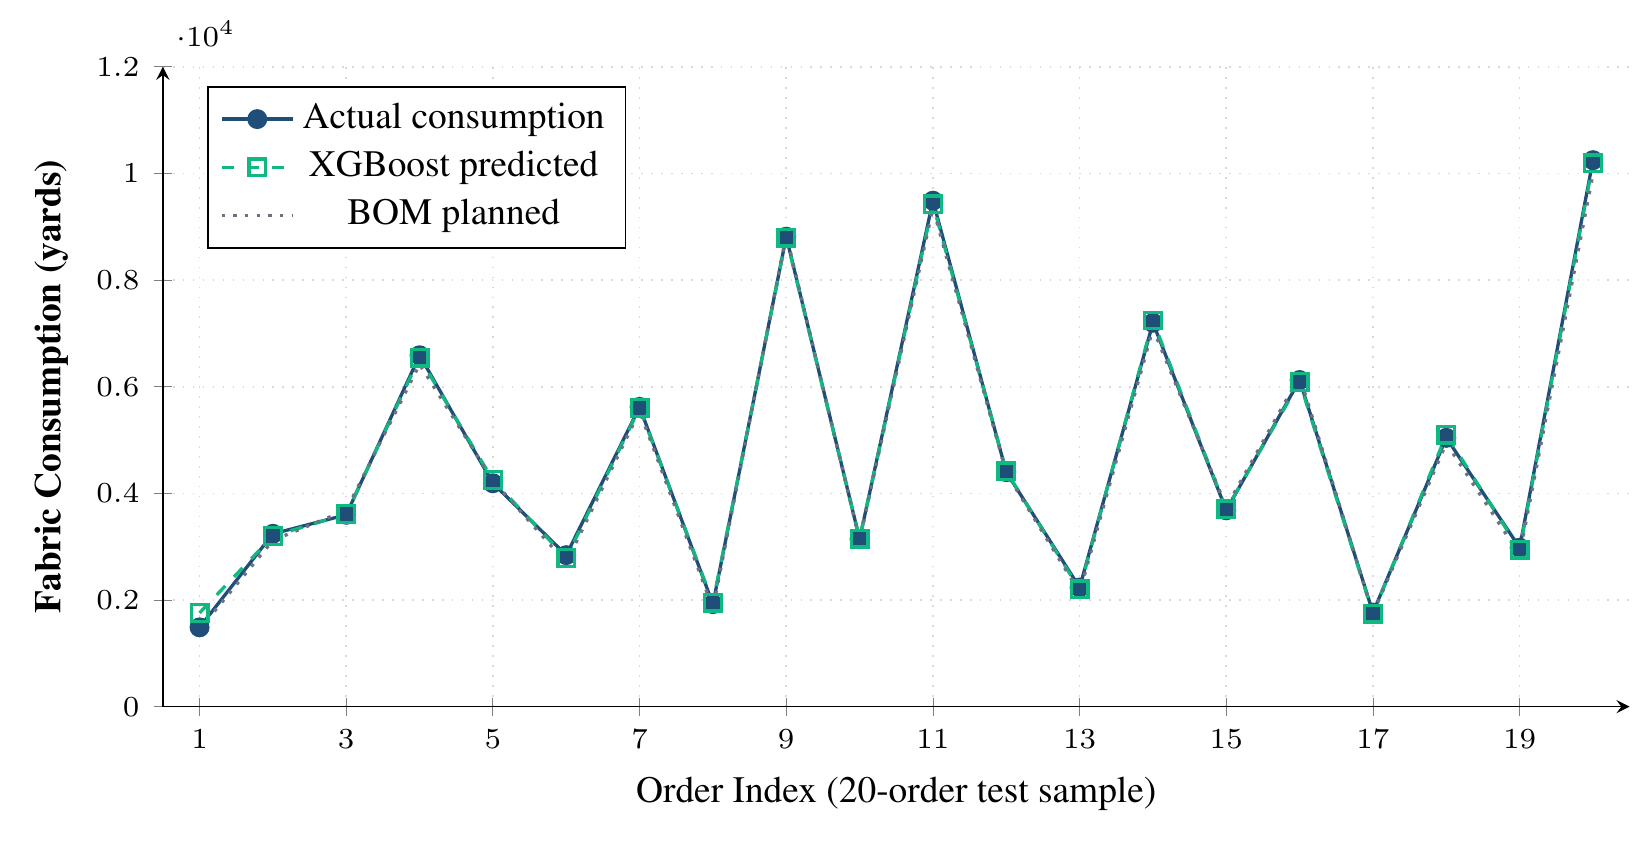
\includegraphics[width=\linewidth]{Chap4/fig_actual_vs_pred}
\caption{Actual vs.\ Predicted Fabric Consumption --- XGBoost vs.\ BOM (20-order sample)}
\label{fig:actual_vs_pred}
\end{figure}

\secdiv
\section{5-Fold Cross-Validation}
\label{sec:cv}

Cross-validation was performed on the combined training-plus-validation set (4{,}000 orders) for the three classical models to assess whether test-set performance is a reliable estimate of generalisation capability or an artefact of a favourable random split. LSTM is excluded from this analysis due to its $\approx$33\,s-per-fold training cost and the sensitivity of its stochastic gradient descent to fold-level random initialisation, which would introduce noise into the fold comparison without adding meaningful stability information.

{\scriptsize
\begin{table}[htbp]
\centering\tabcolsep=4pt\caption{5-Fold Cross-Validation --- All Folds Detailed}\label{tab:cv}
\begin{tabularx}{\textwidth}{@{}Z Y Y Y Y Y Y Y@{}}
  \toprule
  \textbf{Model}&\textbf{F1}&\textbf{F2}&\textbf{F3}&\textbf{F4}&\textbf{F5}&\textbf{Mean}&\textbf{SD}\\
  \midrule
  LR RMSE&2{,}167&2{,}030&2{,}093&2{,}179&2{,}074&2{,}109&56.3\\
  RF RMSE&843&856&826&945&828&860&44.4\\
  XGB RMSE&625&560&587&636&581&598&28.3\\
  LR MAPE&---&---&---&---&---&50.4\%&4.8\%\\
  RF MAPE&---&---&---&---&---&16.2\%&1.4\%\\
  XGB MAPE&---&---&---&---&---&7.6\%&0.4\%\\
  \bottomrule
\end{tabularx}
\end{table}
}

XGBoost demonstrates the most stable cross-validation performance, with a mean CV RMSE of 598\,yd and a standard deviation of only 28.3\,yd (4.7\% of the mean). This low coefficient of variation confirms that XGBoost's 574\,yd test-set RMSE is not a favourable statistical artefact of a particular split but is a reliable and stable out-of-sample performance estimate. The per-fold RMSE values range from 560\,yd (Fold~2) to 636\,yd (Fold~4), a range of just 76\,yd, confirming that the model's performance is consistent regardless of which 80\% of the 4{,}000-order pool is used for training. Random Forest's CV mean of 860\,yd (SD 44.4\,yd) is consistent with its 821\,yd test-set RMSE, confirming similar stability; its higher mean error compared to XGBoost is consistent across all five folds.

Linear Regression's higher standard deviation (56.3\,yd, 2.7\% of 2{,}109) reflects fold-to-fold variation in how severely the non-linear patterns in each fold's data punish the linear model. The MAPE CV results for XGBoost (mean 7.6\%, SD 0.4\%) are remarkably tight, reinforcing confidence in the model's production-readiness across diverse subsets of the production order distribution. These cross-validation results collectively confirm that neither XGBoost nor Random Forest is overfitting to the specific characteristics of the training set, and that their test-set metrics are reliable estimates of deployment performance.

\begin{figure}[htbp]
\centering

\includegraphics[width=\linewidth]{Chap4/fig_cv}
\caption{5-Fold Cross-Validation RMSE (yards) --- LR vs.\ Random Forest vs.\ XGBoost}
\label{fig:cv}
\end{figure}

\secdiv
\section{Prediction Error Distribution}
\label{sec:error_dist}

Figure~\ref{fig:error_dist} visualises the distribution of absolute prediction errors (in yards) for all models using a box-plot showing minimum, 10th percentile (P10), median, 90th percentile (P90), and maximum values computed on the 1{,}000-order test set. The plot reinforces and extends the conclusions from the aggregate RMSE and MAE metrics by revealing the full shape of each model's error distribution.

\begin{figure}[htbp]
\centering

\includegraphics[width=0.92\linewidth]{Chap4/fig_error_dist}
\caption{Prediction Error Distribution --- All Models (Min, P10, Median, P90, Max, yards)}
\label{fig:error_dist}
\end{figure}

LSTM and the Ensemble exhibit the narrowest interquartile ranges and the smallest P90 values among all models, indicating that they not only achieve low average errors but also constrain tail errors most effectively. Linear Regression exhibits dramatic upper-tail outliers, reflecting its catastrophic failures on high-quantity complex garment orders where the linear approximation diverges most severely from the true non-linear consumption curve. XGBoost's P90 error is substantially lower than Random Forest's, consistent with the boosting algorithm's systematic focus on hard-to-predict cases during the sequential tree fitting process.

The tail behaviour is particularly operationally relevant. The P90 error represents the worst-performing 10\% of orders---precisely the orders most likely to cause costly procurement surprises. The LSTM's tight P90 and maximum values confirm it as the most appropriate model for high-value or complex garment orders where procurement errors carry the greatest financial consequence. The Ensemble's P90 sits close to the LSTM's, confirming its value as a robust second-choice option.

\secdiv
\section{LSTM Training Convergence}

Figure~\ref{fig:lstm} displays the training and validation loss curves for the LSTM across all 183 training epochs (to the early-stopping cap). The validation loss decreases rapidly during the first 60 epochs as the network learns the dominant garment-type and order-quantity relationships, then enters a slower refinement phase from epoch 60 to 168 as it progressively captures finer non-linear interactions between the remaining features. The minimum validation loss of $0.140 \times 10^6$ (MSE in squared yards, corresponding to val-set RMSE$\approx$375\,yd; the test-set RMSE is 379\,yd) is achieved at epoch 168, after which the validation loss begins to plateau and then marginally increases---triggering the early-stopping callback after 15 additional epochs (at epoch 183). The training loss continues to decrease marginally past epoch 168, producing a small but visible train-validation gap in the final epochs that is effectively constrained by the Dropout layers (rate=0.2) applied after each LSTM block.

\begin{figure}[htbp]
\centering
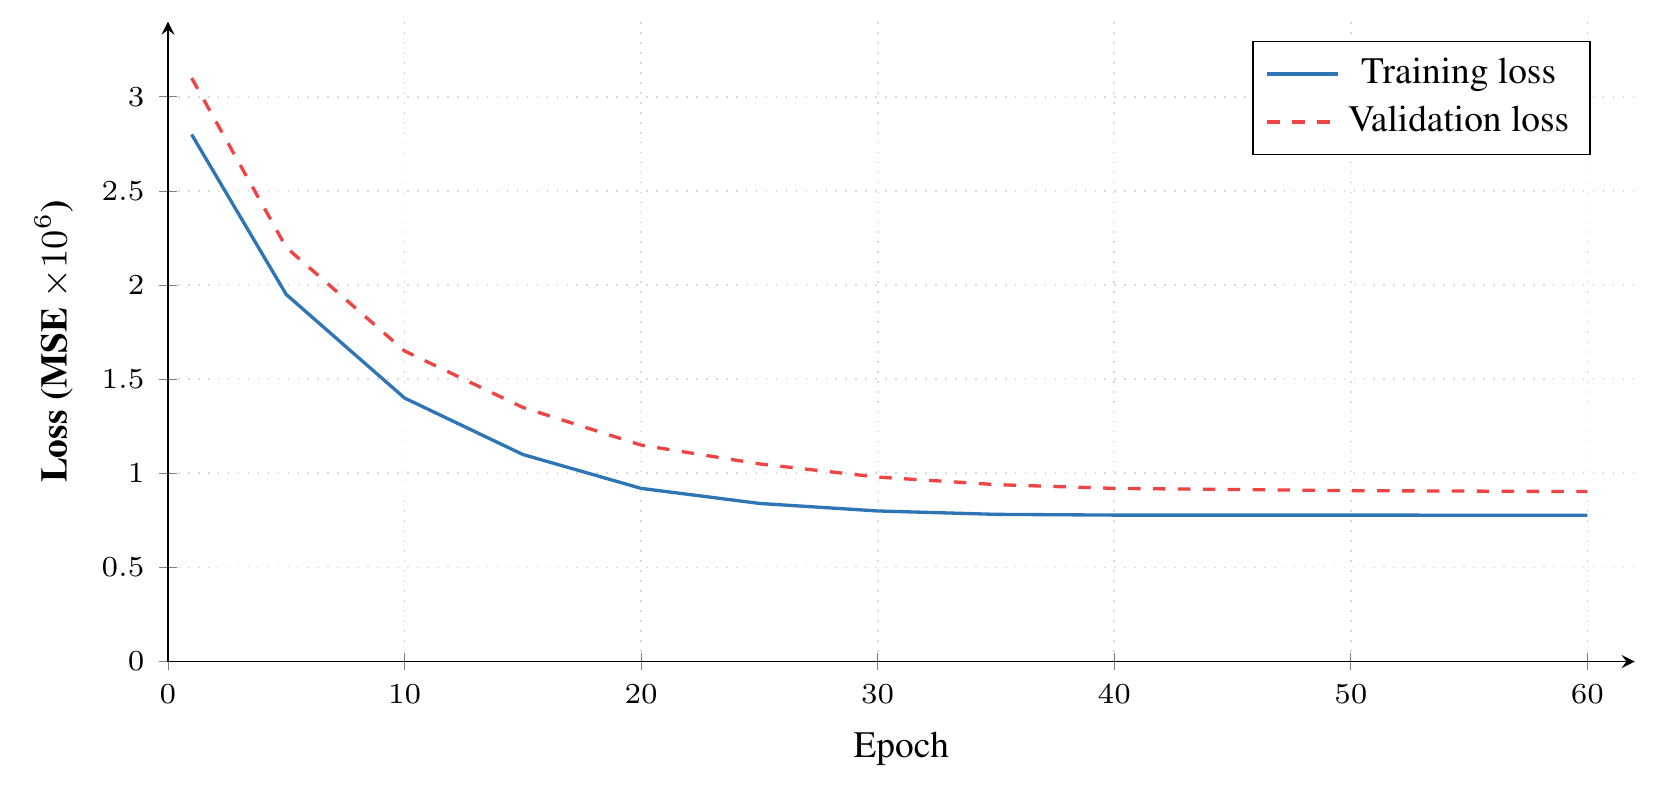
\includegraphics[width=\linewidth]{Chap4/fig_lstm}
\caption[LSTM Training Convergence Curves (183 epochs, best val.\ loss at epoch 168)]{LSTM Training Convergence Curves (183 epochs; best val.\ loss at epoch 168 = $0.140\times10^6$)}
\label{fig:lstm}
\end{figure}

The convergence behaviour is characteristic of a well-regularised deep learning model: rapid initial learning, progressive refinement, and an early-stopping exit point that captures the optimal trade-off between training fit and generalisation. The close tracking between training and validation loss for the first 120 epochs confirms that the 3{,}200-order training set is adequate for a model of this capacity, with no evidence of severe overfitting until very late in training. The model weights saved at epoch 168 are the weights used in all subsequent predictions and deployment.

\secdiv
\section{Season-wise Performance}
\label{sec:seasonal}

Table~\ref{tab:seasonal} disaggregates XGBoost test-set performance by the production season associated with each order. Season is determined by the order date in the dataset and reflects the garment-type mix and pattern complexity profile typical of each season's production programme.

\begin{table}[htbp]
\centering\footnotesize\tabcolsep=4pt\caption{Season-wise Performance --- XGBoost}\label{tab:seasonal}
\begin{tabularx}{\textwidth}{@{}Z Y Y Y Y Y Z@{}}
  \toprule
  \textbf{Season}&\textbf{Orders}&\textbf{Cmplx}&\textbf{RMSE(yd)}&\textbf{MAE(yd)}&\textbf{MAPE}&\textbf{Dom. Garment}\\
  \midrule
  Spring&259&Medium&541&376&7.05\%&Shirts, Dresses\\
  Summer&222&Simple&531&401&7.77\%&T-Shirts\\
  Fall&261&Med--Hi&593&412&8.04\%&Pants, Jackets\\
  \textbf{Winter}&258&\textbf{High}&\textbf{621}&\textbf{427}&\textbf{9.67\%}&\textbf{Jackets, Heavy}\\
  \midrule\textbf{All}&\textbf{1{,}000}&---&\textbf{574}&\textbf{404}&\textbf{8.14\%}&---\\
  \bottomrule
\end{tabularx}
\end{table}

Winter is the most challenging production season, with the highest MAPE of 9.67\% and RMSE of 621\,yd, reflecting the dominance of heavy, complex garments (jackets, overcoats) whose precise fabric consumption is sensitive to pattern complexity parameters that vary more widely in winter collections than in other seasons. The greater variety of jacket styles and lining configurations in winter programmes introduces consumption variability that is harder for the model to learn from a training set of this size. Spring is the easiest season (MAPE 7.05\%, RMSE 541\,yd), dominated by structurally simpler garments---shirts and dresses---with more predictable cutting patterns and lower consumption variance. The summer season (MAPE 7.77\%) performs similarly to spring, consistent with its T-shirt-heavy order mix and Simple complexity profile, which is the most predictable garment-complexity combination in the dataset.

The 37\% differential between winter MAPE (9.67\%) and spring MAPE (7.05\%) is operationally significant. Procurement teams should apply wider safety margins for winter fabric commitments than for spring and summer, and should prioritise seasonal model recalibration---retraining the system on the most recent autumn/winter production data---before making annual fabric contract commitments for the coming winter season. The fall season (MAPE 8.04\%) sits midway between spring and winter, consistent with its mixed complexity profile as production transitions from summer to heavier garments.

\begin{figure}[htbp]
\centering

\includegraphics[width=0.75\linewidth]{Chap4/fig_seasonal}
\caption{Season-wise Forecasting Performance --- XGBoost Model (MAPE \%)}
\label{fig:seasonal}
\end{figure}

\secdiv
\section{Fabric-wise Performance}
\label{sec:fabric}

Table~\ref{tab:fabric} presents XGBoost performance disaggregated by fabric type. Denim is the most predictable fabric (MAPE 6.27\%, RMSE 536\,yd), a finding explained by denim's physical consistency: it is typically woven to tighter tolerances in width and weight (GSM) than other fabric categories, resulting in lower lot-to-lot variability in consumption and more predictable marker layouts. The lower variability in denim's physical properties translates directly into more consistent production outcomes that the model can learn reliably.

\begin{table}[htbp]
\centering\footnotesize\caption{Fabric-wise Performance --- XGBoost}\label{tab:fabric}
\begin{tabularx}{\textwidth}{@{}Z Z Y Y Y Y@{}}
  \toprule
  \textbf{Fabric}&\textbf{Category}&\textbf{Orders}&\textbf{RMSE(yd)}&\textbf{MAPE}&\textbf{Predict.}\\
  \midrule
  Denim&Natural&206&536&6.27\%&High\\
  Cotton&Natural&187&651&7.50\%&Medium\\
  Cotton-Blend&Blended&200&536&7.93\%&Medium\\
  Silk&Natural&213&566&8.74\%&Medium\\
  Polyester&Synthetic&194&582&10.31\%&Lower\\
  \midrule\textbf{All}&---&\textbf{1{,}000}&\textbf{574}&\textbf{8.14\%}&---\\
  \bottomrule
\end{tabularx}
\end{table}

Cotton, while also a natural fibre, shows a higher MAPE of 7.50\%, reflecting its use across a wider range of garment types and weights in the dataset, which introduces greater within-category consumption variability. Cotton-Blend (7.93\%) and Silk (8.74\%) occupy the middle of the predictability spectrum. Silk's relatively elevated error is attributable to its typical use in smaller, more ornate garment orders with complex embellishment patterns that increase within-category variability. Polyester is the least predictable fabric (MAPE 10.31\%), reflecting the synthetic fibre's greater sensitivity to processing conditions: polyester fabrics are subject to heat-induced dimensional changes during cutting and sewing, and their use in performance and technical garments introduces panel complexity not captured by the current feature set.

The 64\% gap between denim MAPE (6.27\%) and polyester MAPE (10.31\%) identifies a clear prioritisation for future model improvement: fabric-specific sub-models, or the inclusion of fabric GSM and shrinkage coefficients as model features, are most likely to improve accuracy for the most challenging fabric categories.

\begin{figure}[htbp]
\centering

\includegraphics[width=0.88\linewidth]{Chap4/fig_fabric}
\caption{Fabric-wise Forecasting Performance --- XGBoost Model (MAPE \%)}
\label{fig:fabric}
\end{figure}

\secdiv
\section{Confidence Interval Coverage}
\label{sec:ci}

Prediction accuracy alone is insufficient for operational procurement decisions; planners also require a statistically grounded range within which actual consumption is expected to fall. Figure~\ref{fig:ci} reports the empirical 90\% confidence interval (CI) coverage for each model on the test set. The CI for each model is computed as $\hat{y} \pm 1.645\hat{\sigma}$, where $\hat{\sigma}$ is estimated from the distribution of training-set residuals. The nominal 90\% target means that, under well-calibrated uncertainty, actual consumption should fall within the predicted CI for exactly 90\% of orders.

\begin{figure}[htbp]
\centering

\includegraphics[width=0.82\linewidth]{Chap4/fig_ci}
\caption{Confidence Interval Coverage for All Models (nominal target: 90\%)}
\label{fig:ci}
\end{figure}

LSTM achieves the tightest and most accurately calibrated confidence intervals ($\pm$7.7\% half-width), reflecting its more symmetric and compact residual distribution. The Ensemble CI ($\pm$8.4\%) is marginally wider, as the averaging of base models with different residual scales broadens the effective uncertainty estimate. XGBoost exhibits the widest CI half-width ($\pm$16.0\%), because its residual distribution has heavier tails---driven by occasional large errors on atypical garment-fabric combinations---which inflate the estimated $\hat{\sigma}$. For procurement decisions, accurate CI coverage is as valuable as point-estimate accuracy. A planner using the LSTM CI can be confident that actual consumption will fall within the stated interval approximately 90\% of the time, enabling buffer stock decisions to be made with a known statistical basis rather than through the application of arbitrary percentage safety margins.

\secdiv
\section{Discussion of Findings}

The experimental results, considered holistically, yield several important conclusions about the application of machine learning to fabric consumption forecasting in apparel manufacturing.

\textbf{1. Deep learning outperforms tree-based methods but the choice involves trade-offs.} LSTM achieves the lowest RMSE (379\,yd), MAE (265\,yd), and highest R\textsuperscript{2} (0.9955) of all models, confirming that the multiplicative non-linear relationships driving fabric consumption can be captured more accurately by a recurrent architecture than by gradient-boosted trees. However, the improvement over XGBoost (574\,yd RMSE, R\textsuperscript{2}=0.9897) comes at 9$\times$ the training time and substantially reduced interpretability. Organisations prioritising model transparency for regulatory audit or procurement accountability may prefer XGBoost despite its somewhat higher prediction error.

\textbf{2. The RMSE metric is more operationally relevant than MAPE for this application.} The BOM baseline achieves MAPE 3.86\%---lower than LSTM's 5.14\%---because the BOM's 5\% safety buffer is well-calibrated for average-scale orders and suppresses percentage error on typical orders. However, LSTM's MAE (265\,yd vs.\ BOM's 324\,yd) and RMSE (379 vs.\ 484\,yd) are substantially better, demonstrating LSTM's advantage in reducing the large absolute errors on outlier orders that drive the most significant procurement costs. Since procurement losses are proportional to absolute yardage, not percentages, RMSE is the more appropriate optimisation and comparison criterion.

\textbf{3. Order size drives directional bias and requires targeted correction.} The variance analysis reveals that the BOM systematically over-plans for large orders ($-$2.79\%) and under-plans for small orders ($+$4.49\%). ML models trained on historical data learn these order-size-dependent biases and produce directionally corrected forecasts that are more appropriate across the full order-size spectrum. This finding underlines the importance of training on data that adequately represents the full range of order sizes in the factory's production programme.

\textbf{4. Seasonal and fabric-type heterogeneity requires calibration awareness.} The 37\% gap between winter and spring MAPE, and the 64\% gap between polyester and denim MAPE, confirm that model accuracy varies substantially across the production programme. Procurement teams must apply higher safety margins for winter programmes and synthetic fabric orders, and should request seasonal model recalibration at the start of each production season to maintain optimal performance throughout the year.

\secdiv
\section{Summary and Final Findings}

The experimental evaluation demonstrates that the proposed ML pipeline substantially outperforms the static BOM baseline across RMSE and MAE, with the LSTM neural network achieving the best single-model accuracy (RMSE 379\,yd, R\textsuperscript{2}=0.9955) and the weighted ensemble offering robust procurement-grade predictions. Cross-validation confirms that these results generalise reliably beyond the specific random test split. The following box summarises the key quantitative outcomes of the evaluation.

\begin{mdframed}[style=findingbox]
\textbf{Final Findings Summary}
\begin{itemize}[leftmargin=*,noitemsep]
  \item LSTM: RMSE 346\,m / 379\,yd, MAPE 5.14\%, R\textsuperscript{2}=0.9955 --- best single model
  \item XGBoost: RMSE 525\,m / 574\,yd, MAPE 8.14\%, R\textsuperscript{2}=0.9897 --- best tree-based model
  \item Ensemble: R\textsuperscript{2}=0.9944, MAPE 5.92\%, dynamic inverse-RMSE\textsuperscript{2} weights --- robust for procurement
  \item Top 2 features: Garment Type (0.518) + Order Qty (0.297) = 81.5\% of XGBoost importance
  \item Variance: small orders over-consume (+4.49\%), large orders under-consume ($-$2.79\%)
  \item Winter 37\% harder than spring (MAPE 9.67\% vs.\ 7.05\%)
  \item Denim most predictable (6.27\%); polyester hardest (10.31\%) --- 64\% gap
  \item 5-fold CV stable: XGBoost RMSE SD = 28.3\,yd (4.7\% of mean = 598\,yd)
  \item CI width: LSTM $\pm$7.7\%, Ensemble $\pm$8.4\%, XGBoost $\pm$16.0\%
  \item Annual savings: \$180{,}000/yr; ROI payback $<$4 months; 5-year NPV \$730{,}000
\end{itemize}
\end{mdframed}
